%! Author = paulsen
%! Date = 12.09.23

\begin{frame}{Software}
    \section{Software}\label{sec:software}
\end{frame}


\begin{frame}{Pakete}
    \subsection{Pakete}\label{subsec:pakete}

    Was sind (Software-)Pakete?

    \vspace{0.5cm}
    \begin{quote}
        Eine Paketverwaltung ermöglicht die komfortable Verwaltung von Software, die in Form von Programmpaketen vorliegt
    \end{quote}

    \begin{itemize}
        \item Pakete sind in einem Zentralen Repository hinterlegt
        \item Ermöglicht strukturiertes Updaten
        \item Kein Linux-Einheitliches Paketformat
    \end{itemize}
\end{frame}

\begin{frame}{Pakete}
    \subsection{Varianten}\label{subsec:varianten}

    \begin{enumerate}
        \item Distributions-Spezifische Paketformate
        \item Unabhängige Containerformate
        \item Sonstiges: Appimage, Nativ, Compiliert mit Sourcecode
    \end{enumerate}

    \vspace{0.5cm}
    \begin{exampleblock}<1->{Fun Fact}
        Android hat "APK" als einheitliches Paketformat
    \end{exampleblock}

\end{frame}

\begin{frame}{Spezifische Paketformate}
    \subsubsection{}\label{subsubsec:spezifische-formate}

    \minipage{0.49\textwidth}
        Distributionsspezifische Paketformate die auf System-Level laufen:
        \begin{itemize}
            \item APT
            \item AUR
            \item YUM
            \item \ldots
        \end{itemize}
    \endminipage\hfill
    \minipage{0.49\textwidth}
        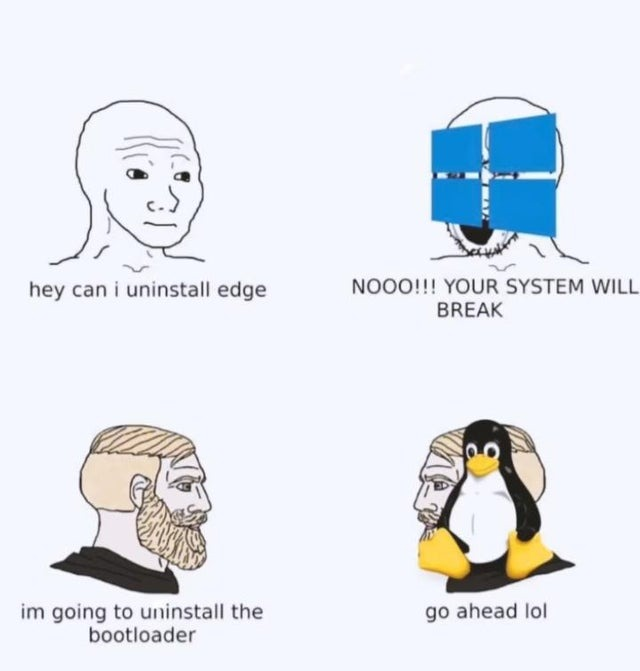
\includegraphics[width=\linewidth]{Meme_Uninstall-Bootloader}
    \endminipage\hfill
\end{frame}

\begin{frame}{Containerformate}
    \subsubsection{}\label{subsubsec:containerformate}

    Laufen System-Unabhängig und meistens auf Benutzer-Level

    \begin{itemize}
        \item Flatpak
        \item Snap
        \item Docker
    \end{itemize}

\end{frame}

\begin{frame}{Sonstige Paketformate}
    \subsubsection{}\label{subsubsec:sonstige-paketformate}

    \begin{itemize}
        \item Appimage: Einzelne Datei beinhaltet die Anwendung und alles was es benötigt
        \item Nativ: Anwendungs-Version ist nur für spezifische Geräteart (ARM-Prozessor, IOS, x86)
        \item Quellcode: Beim Benutzer wird eine (seinem System) zugeschnittene Anwendung erstellt.
    \end{itemize}

\end{frame}

\begin{frame}{Software Installation}
    \subsection{Installation}\label{subsec:installation}

    Discover - TODO

\end{frame}